\section{Mathematical Description}

\label{sec:mathematical-description}

\subsection{Multipole Expansion}

{\color{red} Note: for now this is a copy-paste of JG's g2 note 77 (docdb 3599).  Will edit and make appropriate to the overall length and tone of the paper.}

Polar coordinates ($r,\theta$) in the transverse plane will be adopted in the expressions discussed here, and variations in the longitudinal direction are explicitly assumed to be zero in this section.  See Figure~\ref{fig:coords}.  

\begin{figure}
\begin{center}$
\begin{array}{c}
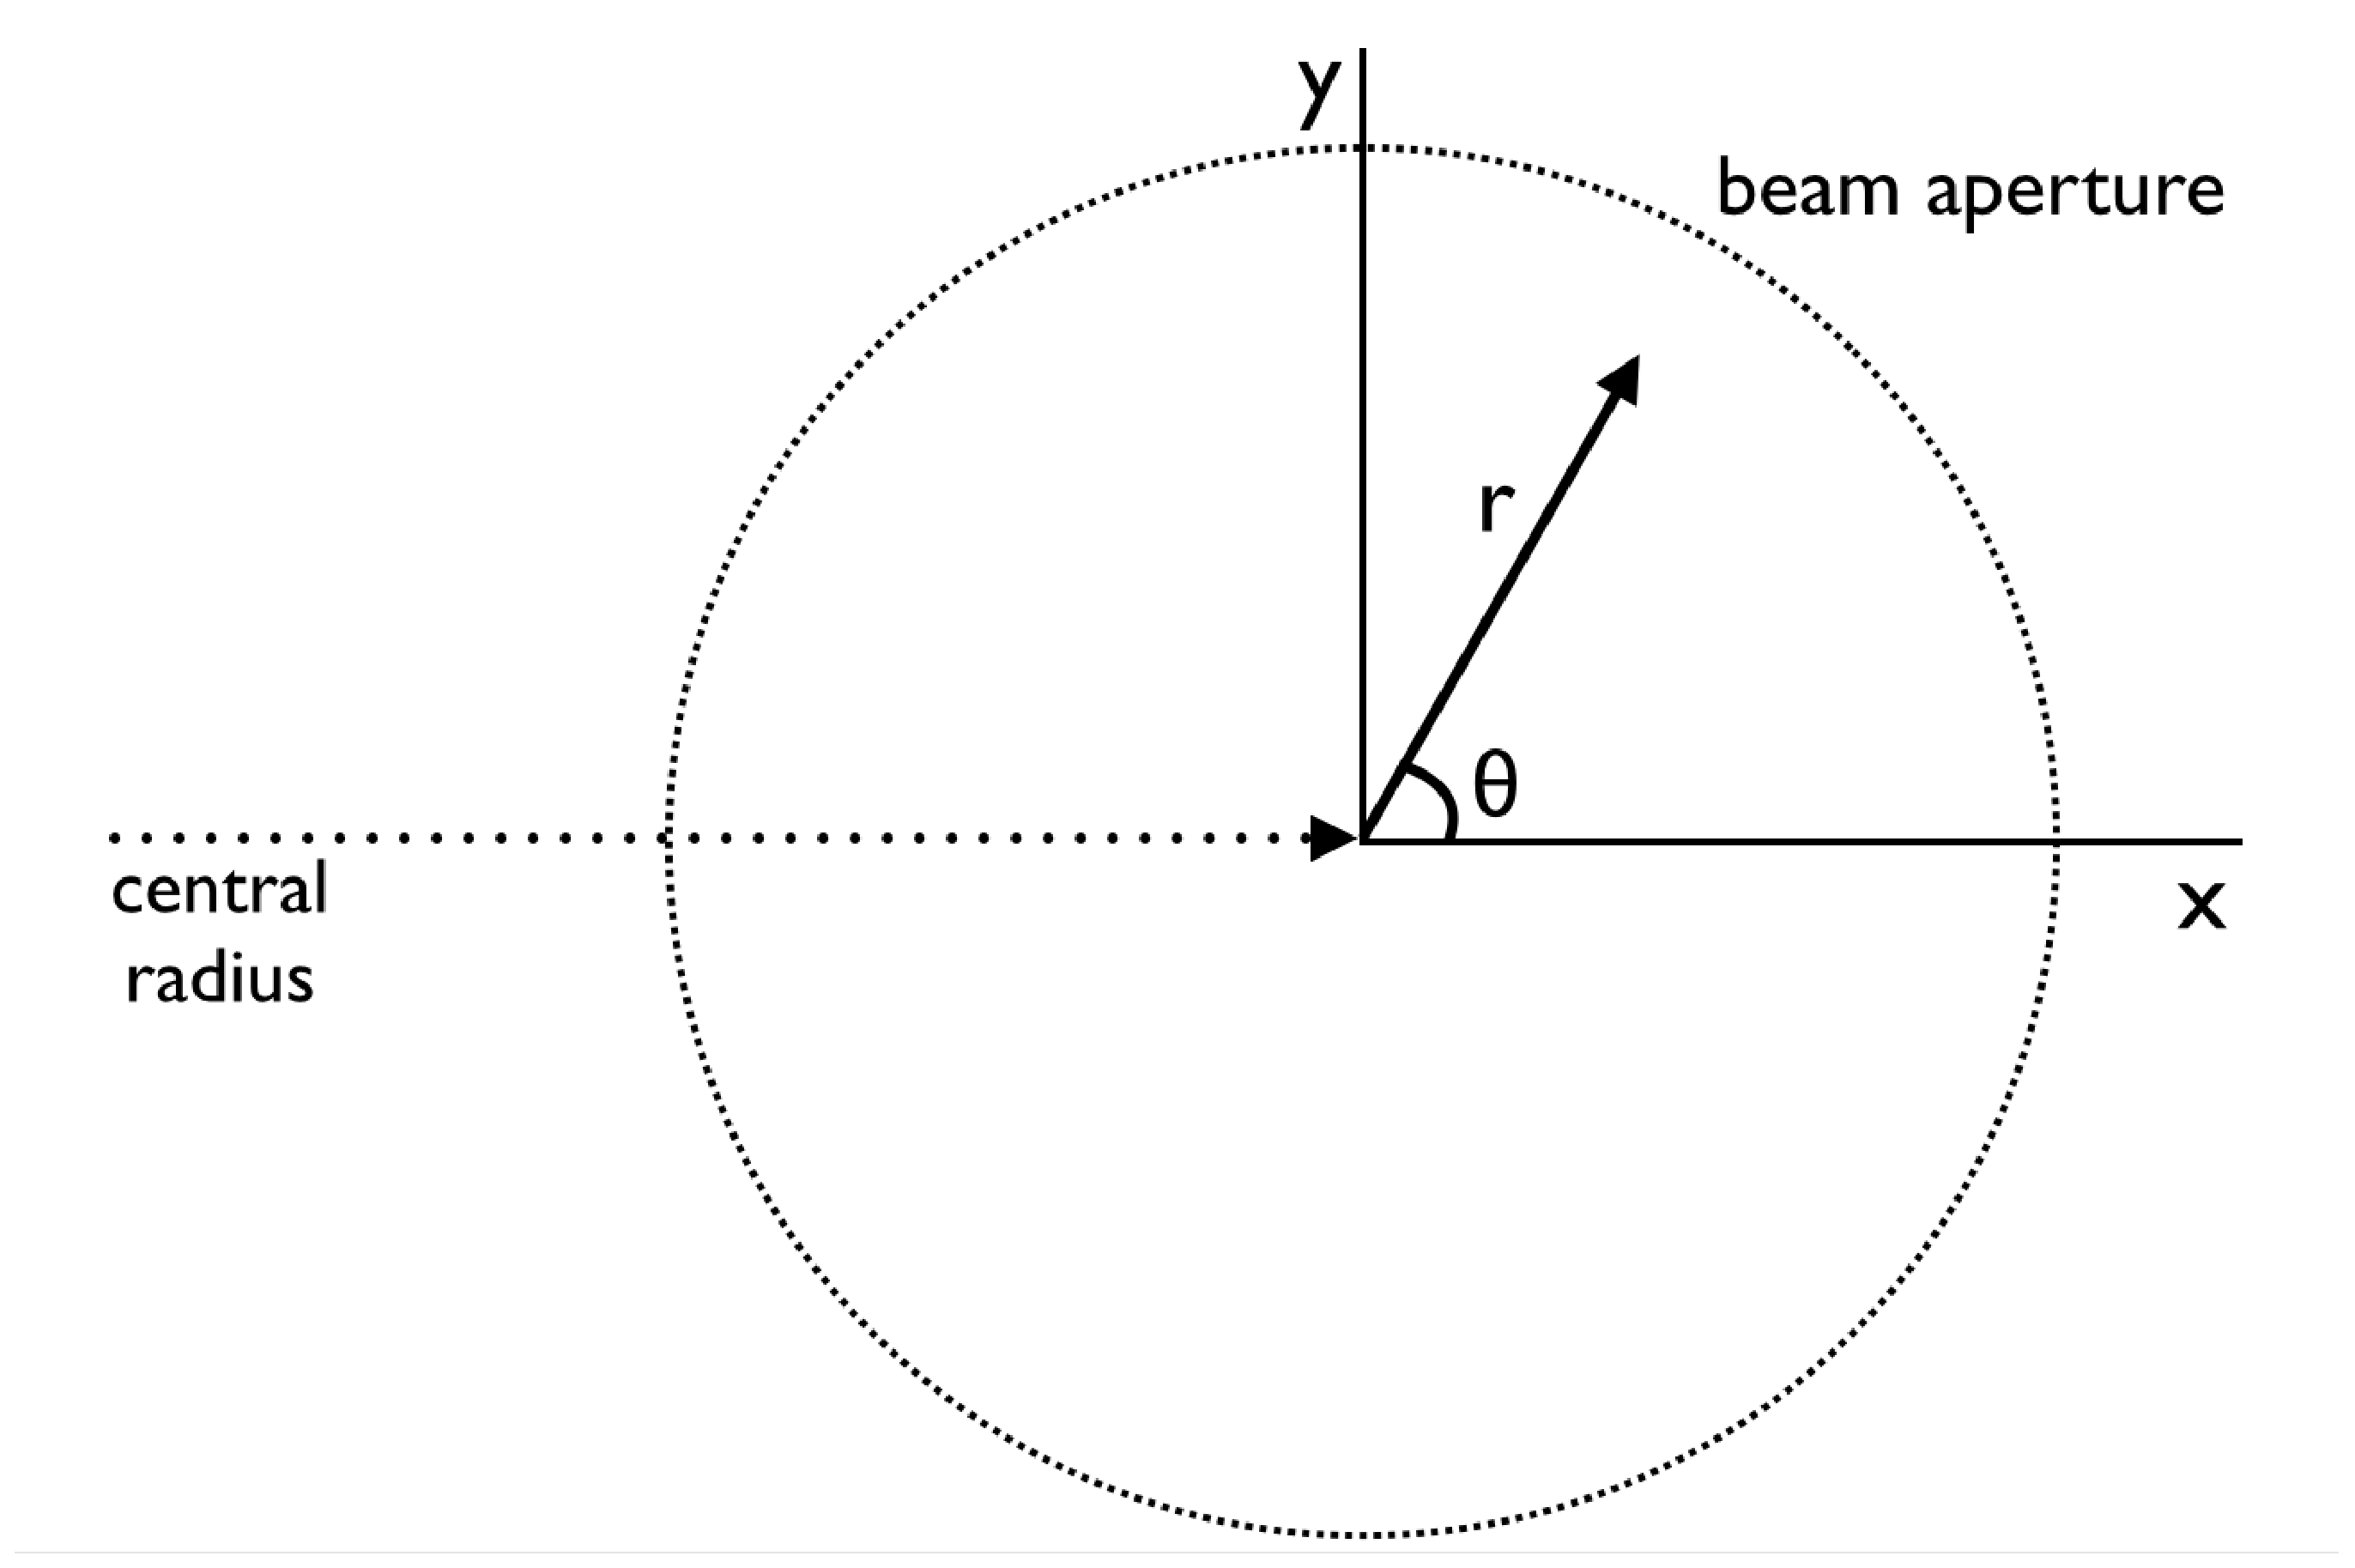
\includegraphics[scale=0.2]{fig/xsec.eps} \\
\end{array}$
\end{center}
\caption{Cartoon of the coordinate system.}
\label{fig:coords} 
\end{figure}

Laplace's equation for a magnetostatic potential $\Phi$ in these coordinates reads:

\begin{center}
\label{eqn:lap}
\begin{eqnarray}
\frac{1}{r}\frac{\partial}{\partial r}\left(r\frac{\partial \Phi}{\partial r} \right) + \frac{1}{r^2}\frac{\partial^2 \Phi}{\partial \theta^2}= 0
\end{eqnarray}
\par\end{center} 

The $r$ and $\theta$ dependence of $\Phi$ may be separated: 

\begin{center}
\begin{eqnarray}
\label{eqn:sep}
\Phi(r,\theta) = R(r)\Theta(\theta)
\end{eqnarray}
\par\end{center} 

So that Equation~\ref{eqn:lap} reduces to:

\begin{center}
\begin{eqnarray}
\frac{1}{\Theta(\theta)}\frac{\partial^2\Theta(\theta)}{\partial \theta^2} = -\frac{r}{R(r)}\frac{\partial}{\partial r}\left(r\frac{\partial R(r)}{\partial r} \right)
\label{eqn:sep2}
\end{eqnarray}
\par\end{center} 

Equation~\ref{eqn:sep2} can be split into two ordinary differential equations related by a separation constant, say $k$, such that:

\begin{center}
\begin{subequations}
\begin{align} 
\frac{1}{\Theta(\theta)}\frac{\partial^2\Theta(\theta)}{\partial \theta^2} = -k^2 \\
\frac{r}{R(r)}\frac{\partial}{\partial r}\left(r\frac{\partial R(r)}{\partial r}\right) = +k^2 .
\end{align}
\label{eqn:sep3}
\end{subequations}
\par\end{center} 

For $k=0$, $R(r) = e\ln r+f$ and $\Theta(\theta) = g\theta+h$, where $e,f,g,h$ are constants.  Since the potential must be defined at the origin, $e=0$.

For $k\neq0$: $R(r) = \alpha r^k + \beta r^{-k}$ and $\Theta(\theta) = \delta \sin (k\theta)+\gamma \cos(k\theta)$ for arbitrary constants $\alpha,\beta,\gamma,\delta$.  Expanding these terms into a power series, the magnetic potential becomes:

\begin{center}
\begin{equation}
\begin{array}{c} 
\Phi(r,\theta) = f(g\theta+h)+\sum\limits_{n=1}^\infty \left[\alpha_n r^{k_n} + \beta_n r^{-k_n}\right]\left[\gamma_n \cos(k_n\theta) + \delta_n \sin(k_n\theta) \right].
\end{array}
\label{eqn:Phi}
\end{equation}
\par\end{center} 

Since $\Phi(r,\theta) = \Phi(r,\theta+2\pi)$, $k_n$ must be an integer.  The potential must also be finite at the origin, so we choose the combination of $\beta_n=0$ and $k_n$ to be a {\it positive} integer.  Then the simplified form of Equation~\ref{eqn:Phi} becomes:

\begin{center}
\begin{equation}
\begin{array}{c} 
\Phi(r,\theta) = f(g\theta+h)+\sum\limits_{n=1}^\infty \alpha_n r^{n}\left[\gamma_n \cos(n\theta) + \delta_n \sin(n\theta) \right].
\end{array}
\label{eqn:PhiRed}
\end{equation}
\par\end{center} 

Now $\vec{B}=-\vec{\nabla}\Phi$, and the $n=0$ term does not contribute to the field: 

\begin{center}
\begin{subequations}
\begin{align} 
B_r = -\frac{\partial \Phi}{\partial r} = -\sum\limits_{n=1}^\infty n \alpha_n r^{n-1}\left[\gamma_n \cos(n\theta) + \delta_n \sin(n\theta) \right] \\
B_\theta = -\frac{1}{r}\frac{\partial \Phi}{\partial \theta} = -\frac{fg}{r}-\sum\limits_{n=1}^\infty n\alpha_n r^{n-1}\left[\delta_n \cos(n\theta) - \gamma_n \sin(n\theta)\right].
\end{align}
\label{eqn:fldcomps}
\end{subequations}
\par\end{center} 

The field must be finite at the origin so $fg=0$.  Since $\hat{r} = \hat{x} \cos \theta + \hat{y} \sin \theta$ and $\hat{\theta} = -\hat{x} \sin \theta + \hat{y} \cos \theta$, Eq.~\ref{eqn:fldcomps} can be expressed in rectangular coordinates:

\begin{center}
\begin{subequations}
\begin{align} 
B_x &= B_r \cos \theta - B_\theta \sin \theta  \\
&= -\sum\limits_{n=1}^\infty n \alpha_n r^{n-1}\left[\left(\gamma_n \cos n\theta + \delta_n \sin n\theta\right) \cos \theta - \left(\delta_n \cos n\theta  - \gamma_n\sin n\theta\right) \sin \theta \right] \\
B_y &= B_r \sin \theta + B_\theta \cos \theta  \\
&= -\sum\limits_{n=1}^\infty n \alpha_n r^{n-1}\left[\left(\gamma_n \cos n\theta + \delta_n \sin n\theta\right) \sin \theta + \left(\delta_n\cos n\theta - \gamma_n \sin n\theta  \right) \cos \theta \right]
\end{align}
\label{eqn:fldcomps4}
\end{subequations}
\par\end{center} 

Using the trigonomic identities:

\begin{center}
\begin{subequations}
\begin{align} 
\cos \alpha \cos \beta \mp \sin \alpha \sin \beta &= \cos (\alpha\pm\beta) \\
\sin \alpha \cos \beta \pm \cos \alpha \sin \beta &= \sin (\alpha\pm\beta), 
\end{align}
\label{eqn:trigid}
\end{subequations}
\par\end{center} 

\noindent and recasting the arbitrary amplitudes $b_n \equiv n\alpha_n \gamma_n$, $a_n \equiv -n\alpha_n \delta_n$ Eq.~\ref{eqn:fldcomps4} becomes:

\begin{center}
\begin{subequations}
\begin{align} 
B_x &= -b_0 + \sum\limits_{n=1}^\infty r^n\left[a_n \sin n\theta - b_n\cos n\theta \right] \\
B_y &= a_0 + \sum\limits_{n=1}^\infty r^n\left[a_n \cos n\theta + b_n\sin n\theta \right]
\end{align}
\label{eqn:fldcomps5}
\end{subequations}
\par\end{center} 

Since NMR cannot resolve the direction of the magnetic field, the effects of $B_x$ and $B_y$ are fully degenerate to the observable signal in NMR.  By construction the vertical field is dominant over the radial field and the quadrature addition of the field components additionally suppresses the contribution of small orthogonal components to the observed quantity $|\vec{B}|$.  To get a feeling for the size of this effect, for the measurement of $b_0$ to be disturbed by the presence of $b_0$ at the level of 10 ppb, $|b_0|$ $\sim$ 150 ppm.  As shown in Fig.~\ref{fig:radfld}, early on in 821 the radial field maximally reached this value.  Since we've restricted the discussion to only two dimensions, azimuthal fields not described here will also play a role.  This will be a significant effect at least near the pole boundaries.
